\documentclass[a4paper,12pt]{article}
\usepackage[english,vietnamese]{babel}
\usepackage[utf8]{inputenc} % Cho phép ký tự UTF-8
\usepackage{amsmath, amssymb}
\usepackage{graphicx}
\usepackage{geometry}
\usepackage{xcolor} % gói để hỗ trợ tô màu
\usepackage[hypertexnames=false,colorlinks=true,linkcolor=black]{hyperref} % Tắt khung đỏ cho mục lục

% Setup cho geometry
\geometry{
 a4paper,
 left=25mm,
 right=25mm,
 top=25mm,
 bottom=25mm,
}

% Setup cho code
\usepackage{listings}
\lstset{
    language=C++,
    basicstyle=\ttfamily\small,
    keywordstyle=\color{blue},
    commentstyle=\color{gray},
    stringstyle=\color{red},
    breaklines=true,
    numbers=left,
    stepnumber=1,
    frame=single,
    literate={_}{\_}1 % chỉ xử lý "_" nếu cần thiết
}



% % Setup cho code
% \lstset{
%   language=C++,
%   basicstyle=\ttfamily,
%   keywordstyle=\color{blue},
%   %commentstyle=\color{gray},
%   stringstyle=\color{red},
%   frame=single,
%   breaklines=true
% }





\title{
    \begin{center}
   
    \Large \textbf{TRƯỜNG ĐẠI HỌC KHOA HỌC TỰ NHIÊN} \\
    \textbf{ĐẠI HỌC QUỐC GIA TP HỒ CHÍ MINH} \\
    \textbf{KHOA CÔNG NGHỆ THÔNG TIN} \\[2cm]
    
\includegraphics[width=0.5\textwidth]{logo.png}\\[2cm] % Điều chỉnh kích thước logo
    \textbf{MÔN HỌC NHẬP MÔN MẬT MÃ - MÃ HÓA}\\
    \textbf{NĂM HỌC 2024 – 2025}\\
    \textbf{HỌC KỲ I}\\
    \textbf{BÁO CÁO ĐỒ ÁN 1}\\
    \textbf{SỐ NGUYÊN TỐ \& TRAO ĐỔI KHÓA DIFFIE-HELLMAN}\\

    \end{center}
}
%\author{Sinh viên: 22120136, 22120141, 22120142, 22120451}
\date{\today}

\begin{document}

\maketitle
\newpage
\tableofcontents
\newpage

\section{Giới thiệu thành viên}
\begin{center}
\begin{tabular}{|l|l|l|l|} % Tạo bảng với 4 cột, các cột được căn trái và có đường viền
\hline % Kẻ đường viền trên cùng của bảng
\textbf{Họ Tên} & \textbf{MSSV} & \textbf{Vai trò} & \textbf{Hoàn thành} \\ \hline
Mai Nhựt Huy & 22120136 & Báo cáo & 0\% \\ \hline
Võ Nguyễn Song Huy & 22120141 & Tạ & 0\% \\ \hline
Vy Quốc Huy & 22120142 & Dev & 0\% \\ \hline
Nguyễn Hùng Việt & 22120451 & Dev & 0\% \\ \hline
\end{tabular}
\end{center}

\section{Giới thiệu bài toán}
Bài báo cáo này trình bày về bài toán số nguyên tố lớn và trao đổi khóa Diffie-Hellman. Mục tiêu là triển khai các thuật toán mật mã cơ bản để tính lũy thừa mô-đun, sinh số nguyên tố an toàn và thực hiện giao thức trao đổi khóa Diffie-Hellman, qua đó hiểu sâu hơn về bảo mật khóa công khai và ứng dụng thực tế.

Quá trình trao đổi khóa Diffie-Hellman gồm các bước sau:

\begin{enumerate}
    \item \textbf{Bước 1: Thiết lập tham số chung}
    \begin{itemize}
        \item Số nguyên tố lớn \( p \) và phần tử sinh \( g \) (giá trị số nguyên, được chọn sao cho có các tính chất toán học đặc biệt liên quan đến số nguyên tố \( p \)) được chia sẻ công khai giữa Alice và Bob. Lý do sử dụng số nguyên tố lớn là để đảm bảo tính bảo mật của thuật toán.
    \end{itemize}
    
    \item \textbf{Bước 2: Sinh khóa riêng của Alice và Bob}
    \begin{itemize}
        \item Khóa riêng của mỗi người (gọi là \( a \) cho Alice và \( b \) cho Bob) được chọn ngẫu nhiên trong khoảng từ \( 2 \) đến \( p-2 \). Khóa riêng này không được tiết lộ cho bất kỳ ai ngoài người dùng.
    \end{itemize}
    
    \item \textbf{Bước 3: Tính khóa công khai và gửi}
    \begin{itemize}
        \item Alice tính khóa công khai \( A = g^a \mod p \) và gửi nó cho Bob.
        \item Tương tự, Bob tính khóa công khai \( B = g^b \mod p \) và gửi nó cho Alice. Khóa công khai này có thể được nhìn thấy bởi mọi người, nhưng vì tính chất toán học của \( g \) và \( p \), khóa riêng \( a \) và \( b \) không thể bị suy ra từ \( A \) và \( B \).
    \end{itemize}
    
    \item \textbf{Bước 4: Tính khóa chung}
    \begin{itemize}
        \item Alice nhận khóa công khai \( B \) từ Bob và tính bí mật chung \( s = B^a \mod p \).
        \item Tương tự, Bob nhận khóa công khai \( A \) từ Alice và tính \( s = A^b \mod p \).
        \item Vì tính chất toán học của phép lũy thừa mô-đun, cả hai người sẽ có cùng một giá trị bí mật chung \( s \) mà không cần tiết lộ khóa riêng của mình. Khóa bí mật chung \( s \) này sẽ được dùng để mã hóa dữ liệu trao đổi giữa Alice và Bob.
    \end{itemize}
\end{enumerate}





\section{Hệ thống xử lý số lớn}

Trong bài tập này, chúng tôi sử dụng một kiểu dữ liệu riêng biệt để xử lý các số nguyên lớn, có thể chứa ít nhất 512 bit. Kiểu dữ liệu này được triển khai dưới dạng lớp \texttt{BigInt}, cho phép thực hiện các phép toán số học cơ bản như cộng, trừ, nhân, chia và các phép toán khác với số nguyên lớn. Lớp \texttt{BigInt} sử dụng mảng ký tự để biểu diễn số nguyên và có thể xử lý cả các số âm và dương.

\subsection{Đặc điểm và các phép toán của lớp \texttt{BigInt}}

\texttt{BigInt} cung cấp một số chức năng chính sau:

\begin{itemize}
    \item \textbf{Khởi tạo:} Lớp \texttt{BigInt} có thể được khởi tạo từ một chuỗi ký tự hoặc từ một số nguyên dài (long long) để biểu diễn số nguyên.
    \item \textbf{Phép toán cộng (+):} Cộng hai số nguyên lớn cùng dấu, nếu khác dấu, chuyển thành phép trừ.
    \item \textbf{Phép toán trừ (-):} Trừ hai số nguyên lớn, xử lý trường hợp số này lớn hơn số kia hay không.
    \item \textbf{Phép toán nhân (*):} Nhân hai số nguyên lớn, với khả năng nhân một số với một hằng số nguyên.
    \item \textbf{Phép toán chia (/):} Chia hai số nguyên lớn, xử lý trường hợp chia cho số 0 và chia cho số 1.
    \item \textbf{Phép toán chia dư (\%):} Tính toán phần dư khi chia hai số nguyên lớn.
    \item \textbf{Các phép toán so sánh:} Các phép toán so sánh như bằng, lớn hơn, nhỏ hơn, khác nhau, v.v... để so sánh giữa các số nguyên lớn.
    \item \textbf{Phép toán dịch trái và phải:} Lớp \texttt{BigInt} cũng hỗ trợ các phép toán dịch trái (\texttt{<<}) và dịch phải (\texttt{>>}) các số nguyên lớn.
\end{itemize}

\subsection{Cấu trúc của lớp \texttt{BigInt}}

Lớp \texttt{BigInt} có các thành phần chính sau:

\begin{itemize}
    \item \textbf{Dấu (Sign):} Lớp sử dụng một kiểu dữ liệu \texttt{enum} để lưu trữ dấu của số (\texttt{positive} hoặc \texttt{negative}).
    \item \textbf{Mảng chứa các chữ số (Digits):} Sử dụng mảng ký tự \texttt{std::vector<char>} để lưu trữ các chữ số của số nguyên lớn, với các chữ số được lưu theo thứ tự ngược lại (từ thấp đến cao).
    \item \textbf{Số chữ số (NumDigits):} Biến \texttt{myNumDigits} lưu số lượng chữ số hiện có trong số nguyên lớn.
\end{itemize}

\subsection{Các hàm thành viên quan trọng của lớp \texttt{BigInt}}

Lớp \texttt{BigInt} bao gồm một số hàm thành viên để thao tác với số nguyên lớn, bao gồm:

\begin{itemize}
    \item \texttt{IsNegative()}: Kiểm tra xem số có phải là số âm hay không.
    \item \texttt{IsPositive()}: Kiểm tra xem số có phải là số dương hay không.
    \item \texttt{NumDigits()}: Trả về số lượng chữ số của số nguyên lớn.
    \item \texttt{GetDigit(int k)}: Lấy chữ số tại vị trí \texttt{k} trong số nguyên.
    \item \texttt{Normalize()}: Làm sạch số, loại bỏ các chữ số 0 thừa.
    \item \texttt{to\_string()}: Chuyển đổi số nguyên lớn thành chuỗi ký tự.
    \item \texttt{lastDigit()}: Lấy chữ số cuối cùng của số nguyên.
\end{itemize}

\subsection{Các toán tử trong lớp \texttt{BigInt}}

Các toán tử cơ bản được định nghĩa trong lớp \texttt{BigInt} như sau:


\begin{itemize}
    \item \verb|BigInt operator + (const BigInt &lhs, const BigInt &rhs);|
    \item \verb|BigInt operator - (const BigInt &lhs, const BigInt &rhs);|
    \item \verb|BigInt operator * (const BigInt &lhs, const BigInt &rhs);|
    \item \verb|BigInt operator / (const BigInt &lhs, const BigInt &rhs);|
    \item \verb|BigInt operator % (const BigInt &lhs, const BigInt &rhs);|
    \item \verb|bool operator == (const BigInt &lhs, const BigInt &rhs);|
    \item \verb|BigInt operator << (const BigInt &lhs, int shift);|
    \item \verb|BigInt operator >> (const BigInt &lhs, int shift);|
    \item \verb|BigInt operator || \verb(const BigInt &lhs, const BigInt &rhs);
\end{itemize}


\subsection{Ví dụ sử dụng}

Dưới đây là một ví dụ sử dụng lớp \texttt{BigInt} trong chương trình:

%                           lỗi khi tạo code C++
\begin{lstlisting}
BigInt a = BigInt("123456789123456789123456789");
BigInt b = BigInt("987654321987654321987654321");
BigInt result = a + b;
std::cout << result.to_string() << std::endl;
\end{lstlisting}

Kết quả sẽ là phép cộng của hai số nguyên lớn và in ra kết quả dưới dạng chuỗi ký tự.















\section{Mô tả và Cài đặt Các Thành Phần}

\subsection{Hàm lũy thừa mô-đun}
Hàm \texttt{modular\_exponentiation} thực hiện tính $(base^{exponent}) \bmod mod$ một cách hiệu quả. Bằng cách lặp lại quá trình lũy thừa mô-đun, ta giảm thiểu số phép tính cần thực hiện.\\

% bug
\begin{lstlisting}
BigInt modular_exponentiation(BigInt base, BigInt exponent, BigInt mod)
{
    BigInt result = 1;
    base = base % mod; // Giam base modulo mod đe tranh tran so

    while (exponent > 0)
    {
        // Neu exponent la so le, nhan voi base
        if (exponent % 2 == 1)
        {
            result = (result * base) % mod;
        }
        // Luy thua nhanh, tang so mu và giam exponent
        base = (base * base) % mod;
        exponent = exponent / 2;
    }

    return result;
}

\end{lstlisting}

\subsection{Sinh số nguyên tố an toàn}
Để sinh số nguyên tố lớn an toàn, chúng tôi sử dụng thuật toán Miller-Rabin. Thuật toán này kiểm tra tính nguyên tố của số dựa vào tính chất số học, giúp đảm bảo rằng số sinh ra là số nguyên tố an toàn.

\begin{lstlisting}
bool miller_rabin(BigInt n, int k = 5)
{
    if (n <= 1 || n == 4)
        return false;
    if (n == 2 || n == 3)
        return true;

    BigInt d = n - 1;
    int r = 0;
    while (d % 2 == 0)
    {
        d = d / 2;
        r++;
    }

    std::random_device rd;
    std::mt19937_64 gen(rd());
    std::uniform_int_distribution<int> dis(2, 100);

    for (int i = 0; i < k; i++)
    {
        BigInt a = dis(gen); // Chọn a ngẫu nhiên
        BigInt x = modular_exponentiation(a, d, n);
        if (x == 1 || x == n - 1)
            continue;
        for (int j = 0; j < r - 1; j++)
        {
            x = (x * x) % n;
            if (x == n - 1)
                break;
        }
        if (x != n - 1)
            return false;
    }
    return true;
}
\end{lstlisting}

\subsection{Sinh khóa riêng}
Khóa riêng cho mỗi bên Alice và Bob được sinh ngẫu nhiên trong khoảng $[2, p-2]$, với $p$ là số nguyên tố đã sinh.

\begin{lstlisting}
BigInt generate_private_key(BigInt p)
{
    random_device rd;
    mt19937_64 gen(rd());
    uniform_int_distribution<int> dis(0, 9);

    BigInt key = 0;
    for (int i = 0; i < p.NumDigits() - 1; ++i)
    {
        key = key * 10 + dis(gen);
    }
    return key % (p - 2) + 2;
}

\end{lstlisting}


\newpage
\section{Phân tích và Đánh giá Kết quả}
\subsection{Kiểm tra tính đúng của bí mật chung}
Kết quả tính toán bí mật chung từ Alice và Bob là trùng khớp, cho thấy quá trình trao đổi khóa đã thành công.
\begin{figure}[h]
    \centering
    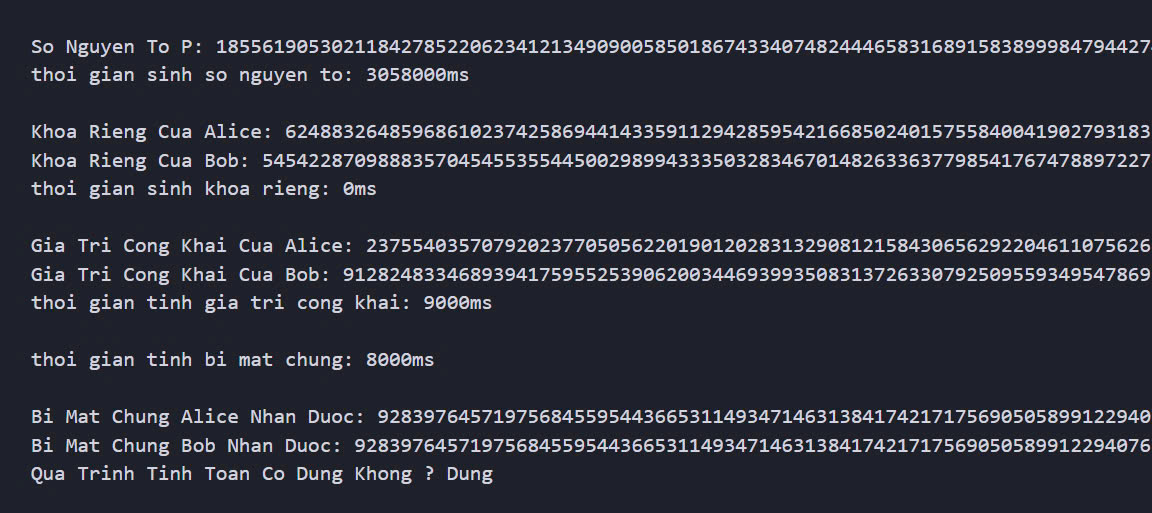
\includegraphics[width=1\textwidth]{output.png}
    \caption{Kết quả tính toán bí mật chung}
    \label{fig:output}
\end{figure}

\subsection{Đánh giá độ phức tạp và hiệu quả}
Các thuật toán đã cài đặt có độ phức tạp hợp lý. Tuy nhiên, có thể tối ưu thêm bằng cách sử dụng thư viện số lớn chuyên biệt.

\subsection{Ứng dụng thực tế của Diffie-Hellman}
Giao thức Diffie-Hellman được sử dụng trong nhiều hệ thống bảo mật, chẳng hạn như SSL/TLS trong giao tiếp web, giúp bảo vệ dữ liệu truyền tải.



\section{Số ngẫu nhiên}
\subsection{Định nghĩa}
Số ngẫu nhiên là một giá trị được tạo ra từ một quy trình ngẫu nhiên, sao cho mỗi số trong một tập hợp các số đều có khả năng xuất hiện như nhau.

\subsection{Độ quan trọng}
Số ngẫu nhiên có vai trò quan trọng và rộng khắp trong nhiều lĩnh vực. Riêng về mật mã học, có rất nhiều cấu trúc mật mã yêu cầu sử dụng số ngẫu nhiên trong cấu trúc:
\begin{itemize}
    \item Giai đoạn tạo khóa của hầu hết các hệ thống mật mã yêu cầu người dùng chọn một hoặc nhiều số ngẫu nhiên (hoặc nguyên tố). Điều này cũng đúng với việc tạo khóa trong hệ thống chữ ký số.
    \item Hệ thống mật mã khóa công khai Elgamal sử dụng một phần tử ngẫu nhiên (số ngẫu nhiên) trong quá trình mã hóa, và các hệ thống chữ ký số kiểu Elgamal như DSA và ECDSA sử dụng phần tử ngẫu nhiên để ký.
    \item Hệ thống mật mã khóa công khai NTRU cũng sử dụng một phần tử ngẫu nhiên trong quá trình mã hóa.
    \item Toàn bộ tiền đề của các phương pháp mã hóa có tính xác suất là kết hợp tính ngẫu nhiên vào quá trình mã hóa.
    \item Hệ thống mật mã hoàn toàn xác định như RSA cũng thu được các tính năng bảo mật quan trọng khi tính ngẫu nhiên được kết hợp vào văn bản gốc.
\end{itemize}

\subsection{Cách tạo một hàm sinh số ngẫu nhiên an toàn}
Để tạo các số ngẫu nhiên an toàn trong môi trường máy tính, cần có một hàm sinh số giả ngẫu nhiên (Pseudorandom Number Generator – PRNG) đáp ứng các yêu cầu bảo mật mật mã. PRNG là một hàm nhận một giá trị đầu vào (seed) và tạo ra một chuỗi bit trông giống như ngẫu nhiên. Chuỗi này cần đảm bảo:
\begin{itemize}
    \item Khả năng dự đoán thấp: nếu một phần chuỗi bit đầu ra của PRNG được biết, kẻ tấn công không thể dự đoán chính xác bit tiếp theo với xác suất cao hơn 50% mà không biết seed ban đầu.
    \item Tính đảo ngược bị giới hạn: ngay cả khi một phần của chuỗi bit bị lộ, kẻ tấn công không thể xác định các giá trị trước đó của chuỗi mà không có seed.
\end{itemize}

Một số phương pháp phổ biến để xây dựng PRNG cho mật mã gồm:
\begin{itemize}
    \item \textbf{Sử dụng Hàm Băm:} Lựa chọn một seed ngẫu nhiên ban đầu và xây dựng chuỗi bằng cách tính toán \( R_i = \text{Hash}(i||S) \) cho mỗi \( i \), trong đó Hash là một hàm băm mật mã như SHA-256. Tuy nhiên, không phải hàm băm nào cũng tạo ra PRNG an toàn, do đó cần chọn kỹ thuật băm đáp ứng yêu cầu bảo mật.
    \item \textbf{Sử dụng Hệ Mã Khóa Đối Xứng:} Các hệ mã như AES hoặc DES có thể được sử dụng để tạo chuỗi bit ngẫu nhiên. Với seed ngẫu nhiên \( S \) và khóa mã hóa \( K \), có thể tạo số ngẫu nhiên từ mã hóa.
\end{itemize}

\section{Xác thực người dùng (Password Authenticated Key Exchange - PAKE) và ứng dụng của Diffie-Hellman}

\subsection{PAKE là gì?}
PAKE (Password Authenticated Key Exchange) là một giao thức bảo mật cho phép xác thực người dùng mà không cần phải gửi mật khẩu qua mạng. Mục tiêu của PAKE là xác minh rằng người dùng có mật khẩu đúng, đồng thời bảo vệ mật khẩu khỏi bị lộ trong suốt quá trình trao đổi thông tin giữa các bên.

\subsection{Lợi ích của PAKE sử dụng Diffie-Hellman}
PAKE sử dụng Diffie-Hellman để tạo ra một khóa chung an toàn mà không tiết lộ mật khẩu qua mạng. Điều này giúp bảo vệ người dùng khỏi các mối đe dọa từ các cuộc tấn công nghe lén (eavesdropping) và tấn công trung gian (MitM). Cụ thể, các lợi ích chính bao gồm:
\begin{itemize}
    \item \textbf{Bảo mật thông tin người dùng:} Mật khẩu không bao giờ được gửi trực tiếp qua mạng, giảm thiểu rủi ro bị đánh cắp qua các cuộc tấn công nghe lén.
    \item \textbf{Chống lại tấn công MitM:} Các cuộc tấn công trung gian không thể giả mạo quá trình trao đổi khóa, vì kẻ tấn công không thể tính toán khóa chung mà không biết mật khẩu chính xác.
    \item \textbf{Đảm bảo tính toàn vẹn và xác thực:} PAKE đảm bảo rằng chỉ những bên có mật khẩu đúng mới có thể thiết lập một kênh giao tiếp an toàn.
    \item \textbf{Bảo vệ khỏi tấn công offline:} Mặc dù kẻ tấn công có thể nắm bắt dữ liệu công khai trao đổi, họ không thể giải mã hoặc đoán mật khẩu từ dữ liệu này, giảm nguy cơ tấn công offline.
\end{itemize}

\subsection{Ứng dụng thực tế của PAKE}
PAKE với Diffie-Hellman có thể được áp dụng trong nhiều tình huống thực tế:
\begin{itemize}
    \item \textbf{Đăng nhập an toàn trên web:} PAKE có thể được sử dụng trong các hệ thống xác thực trực tuyến khi người dùng đăng nhập vào dịch vụ web mà không cần gửi mật khẩu qua mạng, giúp bảo vệ thông tin đăng nhập trong giao thức HTTPS.
    \item \textbf{Hệ thống thanh toán trực tuyến:} PAKE bảo vệ các giao dịch thanh toán trực tuyến, đảm bảo rằng mật khẩu không bị lộ trong suốt quá trình xác thực và bảo vệ giao dịch khỏi các cuộc tấn công.
    \item \textbf{Ứng dụng di động:} Trong các ứng dụng di động, PAKE giúp xác thực người dùng và bảo vệ dữ liệu cá nhân mà không phải tiết lộ mật khẩu qua mạng không an toàn.
\end{itemize}

\subsection{Kết luận}
PAKE sử dụng Diffie-Hellman mang lại giải pháp bảo mật mạnh mẽ cho việc xác thực người dùng, bảo vệ mật khẩu khỏi các cuộc tấn công trực tuyến và giảm thiểu các rủi ro an ninh trong các giao dịch cần trao đổi thông tin nhạy cảm.

\section{Hướng dẫn biên dịch mã nguồn}

1. \textbf{Tải mã nguồn}: Truy cập và tải code từ GitHub qua link:\\ \href{https://github.com/vyquochuy/PRIME-NUMBERS-AND-DIFFIE-HELLMAN-KEY-EXCHANGE}{https://github.com/vyquochuy/\newline PRIME-NUMBERS-AND-DIFFIE-HELLMAN-KEY-EXCHANGE}



2. \textbf{Mở terminal}: Mở terminal tại thư mục \texttt{project\_01\_source} (nơi chứa mã nguồn).

3. \textbf{Biên dịch mã nguồn}: Sử dụng lệnh sau để biên dịch:
\begin{lstlisting}
g++ main.cpp bigInt.cpp -o main
\end{lstlisting}

4. \textbf{Chạy chương trình}: Sau khi biên dịch, chạy chương trình với lệnh:
\begin{lstlisting}
./main
\end{lstlisting}



\section{Kết Luận và Tự Đánh Giá}
Báo cáo đã mô tả các bước triển khai cơ bản và ứng dụng của trao đổi khóa Diffie-Hellman. Nhóm chúng tôi nhận thấy chương trình đã thực hiện đúng các yêu cầu, tuy nhiên có thể cải thiện thêm về hiệu suất và bảo mật.

\appendix
\section{Phụ lục}
Mã nguồn đầy đủ của chương trình và các kết quả kiểm thử.

\end{document}
